\documentclass[a4paper,12pt]{report}
\usepackage{color}
\usepackage{hyperref}
\hypersetup{
    colorlinks,
    citecolor=black,
    filecolor=black,
    linkcolor=black,
    urlcolor=black
}
\setcounter{secnumdepth}{0}
\usepackage{graphicx}
\usepackage{epstopdf}
\epstopdfsetup{outdir=./}
\usepackage{amsmath}
\usepackage[table,xcdraw]{xcolor}
\usepackage{amssymb}
\usepackage{listings}
\definecolor{anti-flashwhite}{rgb}{0.95, 0.95, 0.96}
\lstset{
	language=C++,
    basicstyle=\ttfamily,
    keywordstyle=\color{blue}\ttfamily,
    stringstyle=\color{red}\ttfamily,
	commentstyle=\color{green}\ttfamily,
    morecomment=[l][\color{magenta}]{\#},
    backgroundcolor=\color{anti-flashwhite}
}
\begin{document}
\title{
\textbf{Distributed Computing - II: CS5320}\\~\\
\begin{large}
\textbf{Programming Assignment - I\\~\\External Clock Synchronization
\\~\\}
\end{large}
\begin{large}
\textbf{Assignment Report}
\end{large}
}
\author{\textbf{Sagar Jain - CS17BTECH11034}\\}
\maketitle
\begin{large}
\tableofcontents
\end{large}
\newpage
\section{Program Design}
The following points begin from the \textit{\textbf{main}} function, describing the high level ideas of the code:
\begin{enumerate}
\item Initially we open the I/O files, read input from the files and allocate memory for the data structures used in the code.
\item We then create \textbf{N} threads, each of which simulates one distributed system. This happens in the function \textbf{\textit{serverProcess}}.
\item In each distributed system we have three threads:
\begin{enumerate}
\item Receiver Thread
\item Sender Thread
\item Clock Drift Thread
\end{enumerate}
\item Each server thread first launches threads for receiving and drifting of the clocks.
\item After this the sender thread \textbf{waits for all receiver threads to begin listening}, this is done using a while loop checking the value of a variable, which is being updated by \textbf{reciver thread in the critical section}.
\item The port number given to the ith server is 50000 + i, to make sending requests easier.
\item The sender process then begins sending requests to all the other ports to synchronise with them.
\item \textbf{After one round every sender thread waits for all the other server threads to finish their respective rounds}, so that they can all enter their times into a table at about the same time. This is ensured, again using a \textbf{mutex lock} and variable, whose value is being checked by all the sender threads using a while loop.
\item The receiver thread, sets up a receiving socket and then updates a varibale within a lock so that the sender processes can know when all the receiver threads are ready.
\item The receiver thread on receiving a synchronisation request, get the server id from the message and then responds with the values of T2 and T3, back to the port 50000 + requestinServerID.
\item All the printing to the file happens using \textbf{fprintf} since it does not have the concurrency issues that cout does.
\item We have a class for the localClock of each thread.
\item We finally use the function writeSyncTableToFile, to print the entire table to the file in the requisite format.
\end{enumerate}
\newpage
\section{Program Output}
The program outputa one filea, \textbf{out-log.txt}. The following is an example.\\\\
\textbf{Example Output}:\\\\
\textbf{Log File}:\\\\
\textit{Server 0 replies 1th clock synchronisation response to Server 6 at 00:04:22.\\
Server 1 receives 1th clock synchronisation request from Server 0 at 00:04:22.\\
Server 0 requests 1th clock synchronisation to Server 1 at 00:04:22.\\
Server 5 requests 1th clock synchronisation to Server 0 at 00:04:22.\\
Server 0 receives 2th clock synchronisation request from Server 6 at 00:04:22.\\
Server 3 requests 1th clock synchronisation to Server 0 at 00:04:22.\\
Server 4 receives 1th clock synchronisation response from Server 0 at 00:04:22.\\
Server 0 replies 2th clock synchronisation response to Server 6 at 00:04:22.\\}\\\\

\newpage
\section{Results \& Graphs}
\begin{center}
\begin{large}
\textbf{Variance with Constant Rounds}\\
\end{large}
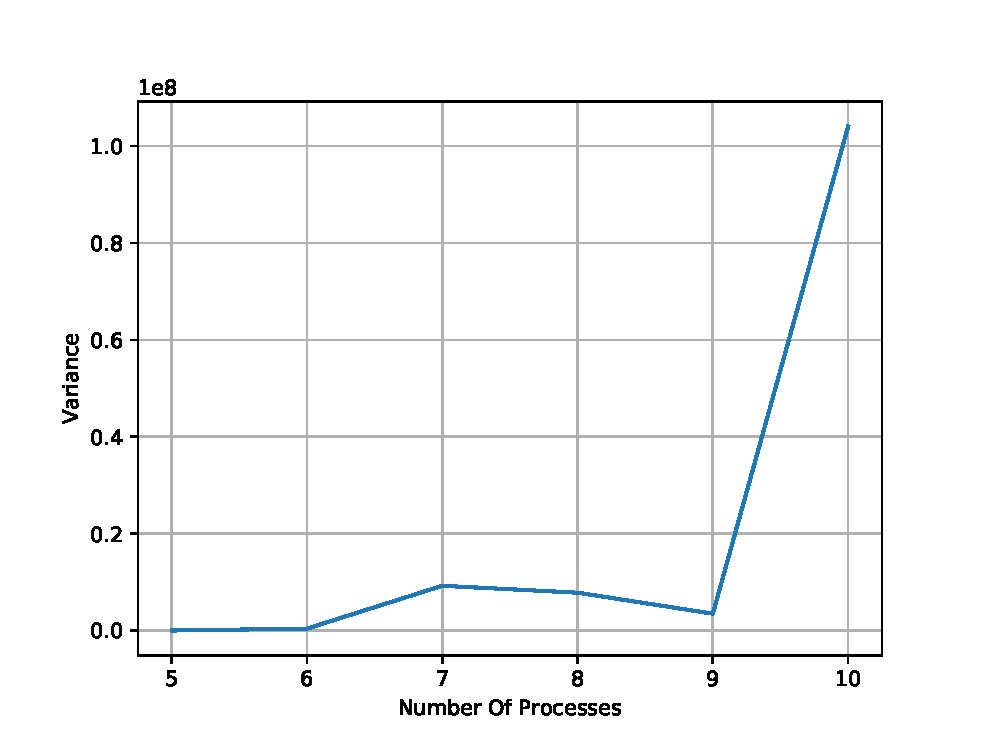
\includegraphics[scale=0.7]{./constantK.eps}
\end{center}
\begin{center}
\begin{large}
\textbf{Variance with Constant Processes}\\
\end{large}
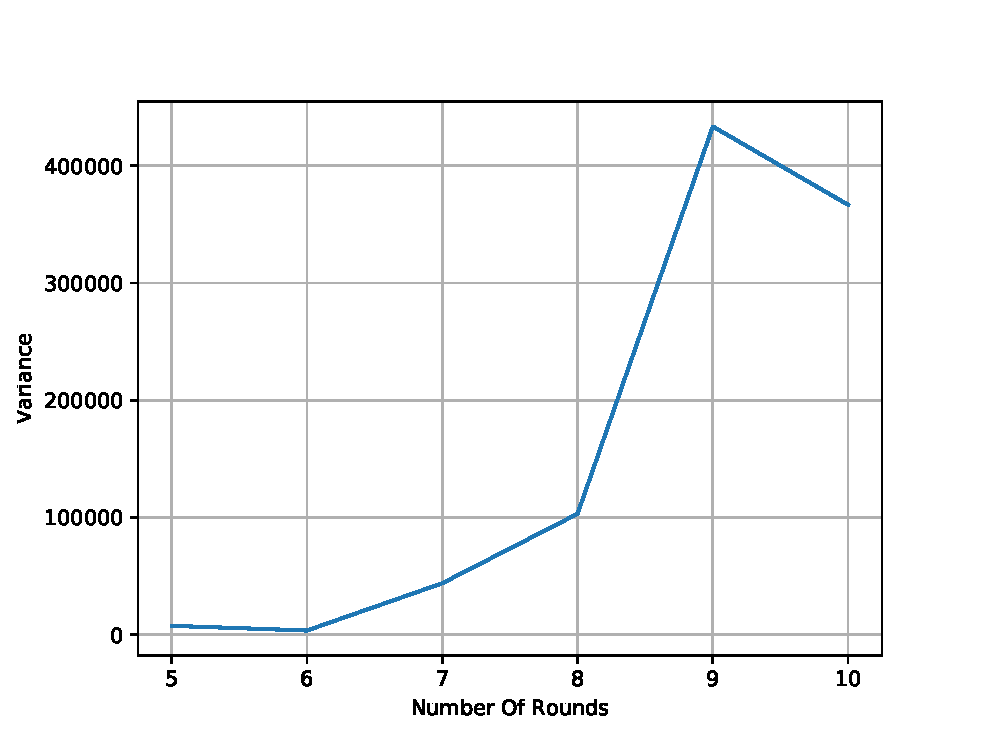
\includegraphics[scale=0.7]{./constantN.eps}
\end{center}

\section{Explaination of Results}
The following are a few points to note / observations about the above graphs:
\begin{enumerate}
\item The first graph shows that with a constant number of rounds the variance is high for a more number of processes. This makes sense, it is due to the fact that while a few processes can be synchronised in less number of rounds, if we would like to synchronise more number of processes we need more rounds of synchronisations.
\item For a constant number of processes we see that initially the variance increases from 0 and then at the end starts to decrease, this happens because of two simple reasons:
\begin{enumerate}
\item Initially the clocks are actually in-sync as they are all the system clock, so the initial variance is 0, but with increase in time, the drift and unnecessary accounting for round trip times begins to diverge the clocks, so we see the clock variance increasing.
\item As the rounds increase, the synchronisation begins to take place so we see that at the end the variance begins to decrease.
\end{enumerate}
\end{enumerate}
\end{document}